\documentclass[english,man]{apa6}

\usepackage{amssymb,amsmath}
\usepackage{ifxetex,ifluatex}
\usepackage{fixltx2e} % provides \textsubscript
\ifnum 0\ifxetex 1\fi\ifluatex 1\fi=0 % if pdftex
  \usepackage[T1]{fontenc}
  \usepackage[utf8]{inputenc}
\else % if luatex or xelatex
  \ifxetex
    \usepackage{mathspec}
    \usepackage{xltxtra,xunicode}
  \else
    \usepackage{fontspec}
  \fi
  \defaultfontfeatures{Mapping=tex-text,Scale=MatchLowercase}
  \newcommand{\euro}{€}
\fi
% use upquote if available, for straight quotes in verbatim environments
\IfFileExists{upquote.sty}{\usepackage{upquote}}{}
% use microtype if available
\IfFileExists{microtype.sty}{\usepackage{microtype}}{}

% Table formatting
\usepackage{longtable, booktabs}
\usepackage{lscape}
% \usepackage[counterclockwise]{rotating}   % Landscape page setup for large tables
\usepackage{multirow}		% Table styling
\usepackage{tabularx}		% Control Column width
\usepackage[flushleft]{threeparttable}	% Allows for three part tables with a specified notes section
\usepackage{threeparttablex}            % Lets threeparttable work with longtable

% Create new environments so endfloat can handle them
% \newenvironment{ltable}
%   {\begin{landscape}\begin{center}\begin{threeparttable}}
%   {\end{threeparttable}\end{center}\end{landscape}}

\newenvironment{lltable}
  {\begin{landscape}\begin{center}\begin{ThreePartTable}}
  {\end{ThreePartTable}\end{center}\end{landscape}}

  \usepackage{ifthen} % Only add declarations when endfloat package is loaded
  \ifthenelse{\equal{\string man}{\string man}}{%
   \DeclareDelayedFloatFlavor{ThreePartTable}{table} % Make endfloat play with longtable
   % \DeclareDelayedFloatFlavor{ltable}{table} % Make endfloat play with lscape
   \DeclareDelayedFloatFlavor{lltable}{table} % Make endfloat play with lscape & longtable
  }{}%



% The following enables adjusting longtable caption width to table width
% Solution found at http://golatex.de/longtable-mit-caption-so-breit-wie-die-tabelle-t15767.html
\makeatletter
\newcommand\LastLTentrywidth{1em}
\newlength\longtablewidth
\setlength{\longtablewidth}{1in}
\newcommand\getlongtablewidth{%
 \begingroup
  \ifcsname LT@\roman{LT@tables}\endcsname
  \global\longtablewidth=0pt
  \renewcommand\LT@entry[2]{\global\advance\longtablewidth by ##2\relax\gdef\LastLTentrywidth{##2}}%
  \@nameuse{LT@\roman{LT@tables}}%
  \fi
\endgroup}


  \usepackage{graphicx}
  \makeatletter
  \def\maxwidth{\ifdim\Gin@nat@width>\linewidth\linewidth\else\Gin@nat@width\fi}
  \def\maxheight{\ifdim\Gin@nat@height>\textheight\textheight\else\Gin@nat@height\fi}
  \makeatother
  % Scale images if necessary, so that they will not overflow the page
  % margins by default, and it is still possible to overwrite the defaults
  % using explicit options in \includegraphics[width, height, ...]{}
  \setkeys{Gin}{width=\maxwidth,height=\maxheight,keepaspectratio}
\ifxetex
  \usepackage[setpagesize=false, % page size defined by xetex
              unicode=false, % unicode breaks when used with xetex
              xetex]{hyperref}
\else
  \usepackage[unicode=true]{hyperref}
\fi
\hypersetup{breaklinks=true,
            pdfauthor={},
            pdftitle={R you ready to write a paper in R Markdown?},
            colorlinks=true,
            citecolor=blue,
            urlcolor=blue,
            linkcolor=black,
            pdfborder={0 0 0}}
\urlstyle{same}  % don't use monospace font for urls

\setlength{\parindent}{0pt}
%\setlength{\parskip}{0pt plus 0pt minus 0pt}

\setlength{\emergencystretch}{3em}  % prevent overfull lines

\ifxetex
  \usepackage{polyglossia}
  \setmainlanguage{}
\else
  \usepackage[english]{babel}
\fi

% Manuscript styling
\captionsetup{font=singlespacing,justification=justified}
\usepackage{csquotes}
\usepackage{upgreek}

 % Line numbering
  \usepackage{lineno}
  \linenumbers


\usepackage{tikz} % Variable definition to generate author note

% fix for \tightlist problem in pandoc 1.14
\providecommand{\tightlist}{%
  \setlength{\itemsep}{0pt}\setlength{\parskip}{0pt}}

% Essential manuscript parts
  \title{R you ready to write a paper in R Markdown?}

  \shorttitle{R you ready}


  \author{Rick O. Gilmore\textsuperscript{1,2}~\& Michael Hallquist\textsuperscript{1}}

  % \def\affdep{{"", ""}}%
  % \def\affcity{{"", ""}}%

  \affiliation{
    \vspace{0.5cm}
          \textsuperscript{1} The Pennsylvania State University\\
          \textsuperscript{2} Databrary.org  }

  \authornote{
    The authors are with the Department of Psychology at The Pennsylvania
    State University. The authors acknowledge support from the Department of
    Psychology, the Social, Life, \& Engineering Sciences Imaging Center
    (SLEIC), and the Child Study Center's Open Data in Developmental Science
    (ODDS) initiative.
    
    Correspondence concerning this article should be addressed to Rick O.
    Gilmore, Department of Psychology, The Pennsylvania State University,
    University Park, PA 16802 USA. E-mail:
    \href{mailto:rogilmore@psu.edu}{\nolinkurl{rogilmore@psu.edu}}
  }


  \abstract{Want to write a paper using R Markdown? Keep reading to see how.}
  \keywords{APA, R Markdown \\

    \indent Word count: Not that many.
  }





\usepackage{amsthm}
\newtheorem{theorem}{Theorem}[section]
\newtheorem{lemma}{Lemma}[section]
\theoremstyle{definition}
\newtheorem{definition}{Definition}[section]
\newtheorem{corollary}{Corollary}[section]
\newtheorem{proposition}{Proposition}[section]
\theoremstyle{definition}
\newtheorem{example}{Example}[section]
\theoremstyle{definition}
\newtheorem{exercise}{Exercise}[section]
\theoremstyle{remark}
\newtheorem*{remark}{Remark}
\newtheorem*{solution}{Solution}
\begin{document}

\maketitle

\setcounter{secnumdepth}{0}



It is possible to write an entire APA-formatted article in R Markdown.
This very brief paper shows how it might be done. As illustration, we
use the data from a short, informal survey of participants in the 2018 R
Bootcamp at Penn State.

\section{Methods}\label{methods}

Consistent with open and transparent science practices, we report how we
determined our sample size, all data exclusions (if any), all
manipulations, and all measures in the study (Simmons, Nelson, \&
Simonsohn, 2011).

\subsection{Participants}\label{participants}

We asked participants in an optional \enquote{R Bootcamp} held at the
Pennsylvania State University Department of Psychology on August 16 and
17, 2018 to complete an anonymous survey using a Google Form. We asked
participants to report how old they felt. A total of \(n=\) 56
respondents answered the survey with a reported felt age of \(M\)=50.75
and a range of {[}5-1000{]} years.

\subsection{Material}\label{material}

The survey can be found at this URL:
\url{https://docs.google.com/forms/d/e/1FAIpQLSeGqic9Hrj-XvkESZmu_0t6H02R-U6yzYnRLuX6HDFDp4R39g/viewform}.
There were six questions asked:

\begin{enumerate}
\def\labelenumi{\arabic{enumi}.}
\tightlist
\item
  Your current level of experience/expertise with R
\item
  Your enthusiasm for banjo music?
\item
  How old do you feel (in years)?
\item
  Preferred number of hours spent sleeping/day
\item
  Favorite day of the week?
\item
  Is there a reproducibility \enquote{crisis} in psychology?
\end{enumerate}

\subsection{Procedure}\label{procedure}

We emailed a link to the survey to the list of participants in advance.
We also include a link to the survey on the web page containing the
course schedule
(\url{https://psu-psychology.github.io/r-bootcamp-2018/schedule.html}).
We encouraged participants to complete the survey before the first day
or during lunch.

\subsection{Data analysis}\label{data-analysis}

We used R (Version 3.5.1; R Core Team, 2018) and the R-packages
\emph{afex} (Version 0.21.2; Singmann, Bolker, Westfall, \& Aust, 2018),
\emph{bindrcpp} (Version 0.2.2; Müller, 2018), \emph{dataMaid} (Version
1.1.2; Petersen \& Ekstrøm, 2018), \emph{dplyr} (Version 0.7.6; Wickham,
François, Henry, \& Müller, 2018), \emph{emmeans} (Version 1.2.3; Lenth,
2018), \emph{forcats} (Version 0.3.0; Wickham, 2018a), \emph{Formula}
(Version 1.2.3; Zeileis \& Croissant, 2010), \emph{ggplot2} (Version
3.0.0; Wickham, 2016), \emph{gmodels} (Version 2.18.1; Warnes et al.,
2018), \emph{googlesheets} (Version 0.3.0; Bryan \& Zhao, 2018),
\emph{haven} (Version 1.1.2; Wickham \& Miller, 2018), \emph{Hmisc}
(Version 4.1.1; Harrell Jr, Charles Dupont, \& others., 2018),
\emph{lattice} (Version 0.20.35; Sarkar, 2008), \emph{lme4} (Version
1.1.17; Bates, Mächler, Bolker, \& Walker, 2015), \emph{Matrix} (Version
1.2.14; Bates \& Maechler, 2018), \emph{pander} (Version 0.6.2; Daróczi
\& Tsegelskyi, 2018), \emph{papaja} (Version 0.1.0.9709; Aust \& Barth,
2018), \emph{purrr} (Version 0.2.5; Henry \& Wickham, 2018),
\emph{readr} (Version 1.1.1; Wickham, Hester, \& Francois, 2017),
\emph{stringr} (Version 1.3.1; Wickham, 2018b), \emph{survival} (Version
2.42.6; Terry M. Therneau \& Patricia M. Grambsch, 2000), \emph{tibble}
(Version 1.4.2; Müller \& Wickham, 2018), \emph{tidyr} (Version 0.8.1;
Wickham \& Henry, 2018), \emph{tidyverse} (Version 1.2.1; Wickham,
2017), and \emph{tufte} (Version 0.4; Xie \& Allaire, 2018) for all our
analyses. The code used to generate these analyses is embedded in this
document. To view it, see the R Markdown file in the
\href{http://github.com/psu-psychology/r-bootcamp-2018/talks}{GitHub
repository} associated with this paper.

\section{Results}\label{results}

\begin{table}[tbp]
\begin{center}
\begin{threeparttable}
\caption{\label{tab:Banjo-by-experience}Descriptive statistics of banjo music enthusiasm by R experience.}
\begin{tabular}{llllll}
\toprule
R\_exp & \multicolumn{1}{c}{Mean} & \multicolumn{1}{c}{Median} & \multicolumn{1}{c}{SD} & \multicolumn{1}{c}{Min} & \multicolumn{1}{c}{Max}\\
\midrule
none & 3.90 & 4.00 & 2.08 & 1.00 & 7.00\\
limited & 4.75 & 4.00 & 3.05 & 1.00 & 10.00\\
lots & 4.09 & 3.00 & 2.02 & 1.00 & 7.00\\
pro & 6.00 & 6.00 & 5.66 & 2.00 & 10.00\\
NA & 1.00 & 1.00 & NA & 1.00 & 1.00\\
\bottomrule
\addlinespace
\end{tabular}
\begin{tablenotes}[para]
\textit{Note.} This table was created with apa\_table()
\end{tablenotes}
\end{threeparttable}
\end{center}
\end{table}

\begin{table}[tbp]
\begin{center}
\begin{threeparttable}
\caption{\label{tab:apa-corr-table}Correlation table of the example data set.}
\begin{tabular}{lll}
\toprule
 & \multicolumn{1}{c}{Banjo} & \multicolumn{1}{c}{Psych\_age\_yrs}\\
\midrule
Banjo &  & \\
Psych\_age\_yrs & -0.15 & \\
Sleep\_hrs & 0.06 & 0.59***\\
\bottomrule
\addlinespace
\end{tabular}
\begin{tablenotes}[para]
\textit{Note.} This is a correlation table created using apa\_table().
\end{tablenotes}
\end{threeparttable}
\end{center}
\end{table}

\begin{figure}
\centering
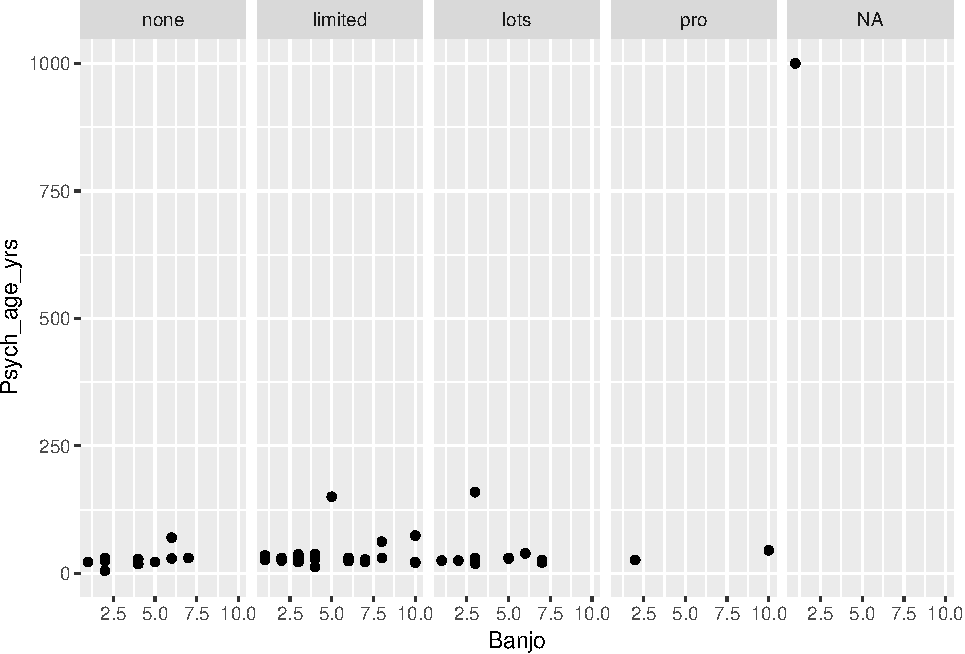
\includegraphics{gilmore-hallquist-bootcamp-2018-papaja_files/figure-latex/Banjo-by-age-exp-1.pdf}
\caption{\label{fig:Banjo-by-age-exp}Banjo music enthusiasm by age and R
experience}
\end{figure}

\begin{figure}
\centering
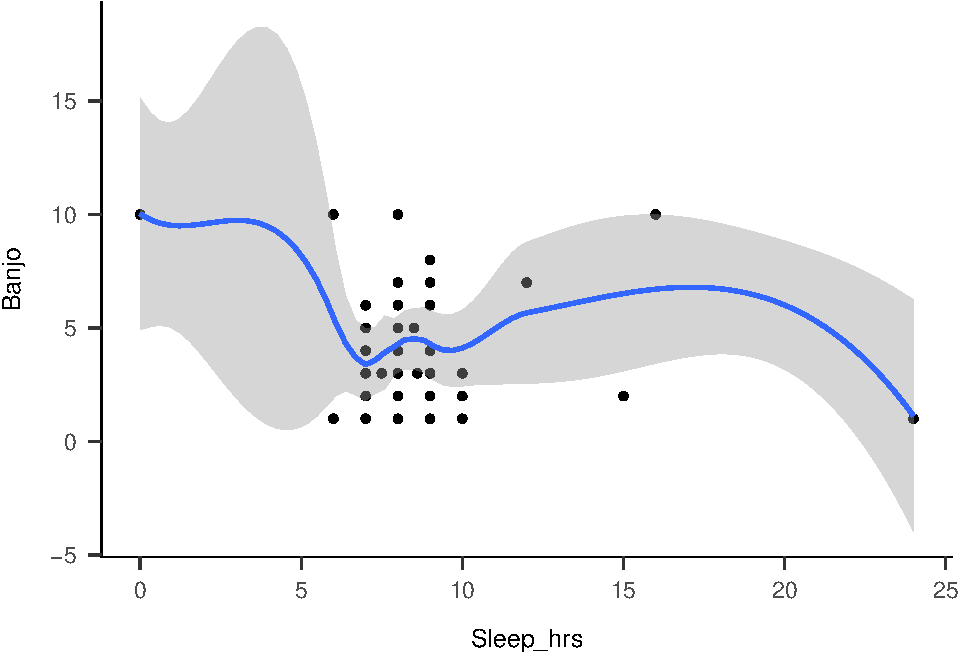
\includegraphics{gilmore-hallquist-bootcamp-2018-papaja_files/figure-latex/Banjo-by-sleep-1.pdf}
\caption{\label{fig:Banjo-by-sleep}Banjo music enthusiasm by preferred hours
of sleep}
\end{figure}

\begin{table}[tbp]
\begin{center}
\begin{threeparttable}
\caption{\label{tab:Banjo-aov-table}ANOVA table for the analyis of the example data set.}
\begin{tabular}{lrcrrrl}
\toprule
Effect & \multicolumn{1}{c}{$F$} & \multicolumn{1}{c}{$\mathit{df}_1$} & \multicolumn{1}{c}{$\mathit{df}_2$} & \multicolumn{1}{c}{$\mathit{MSE}$} & \multicolumn{1}{c}{$p$} & \multicolumn{1}{c}{$\hat{\eta}^2_p$}\\
\midrule
R exp & 0.51 & 3 & 51 & 7.84 & .679 & .029\\
\bottomrule
\addlinespace
\end{tabular}
\begin{tablenotes}[para]
\textit{Note.} This is a table created using apa\_print() and apa\_table().
\end{tablenotes}
\end{threeparttable}
\end{center}
\end{table}

Table \ref{tab:Banjo-by-experience} summarizes the banjo music
enthusiasm ratings data by levels of R experience. As Gilmore predicted,
the more participants know about R, the more they come to appreciate
banjo music.

Let's examine the correlations between our continuous variables. As
indicated in Table \ref{tab:apa-corr-table}, there is a non-significant
negative correlation (\(r = -.15\), 95\% CI \([-.40\), \(.12]\)) between
banjo music enthusiasm and age (\(t(54) = -1.10\), \(p = .275\)), no
correlation (\(r = .06\), 95\% CI \([-.21\), \(.31]\)) between banjo
music enthusiasm and sleep (\(t(54) = 0.41\), \(p = .683\)), but a
positive correlation (\(r = .59\), 95\% CI \([.39\), \(.74]\)) between
age and sleep (\(t(54) = 5.44\), \(p < .001\)). Figures
\ref{fig:Banjo-by-age-exp} and \ref{fig:Banjo-by-sleep} depict these
patterns.

To test the hypothesis that banjo music enthusiasm varies as a function
of R expertise, we carried out a one-way ANOVA. R experience
(\(F(3, 51) = 0.51\), \(\mathit{MSE} = 7.84\), \(p = .679\),
\(\hat{\eta}^2_p = .029\)) did not predict enthusiasm for banjo music,
so Gilmore will have to continue searching for userRs who appreciate the
banjo. Table \ref{tab:Banjo-aov-table} summarizes these results.

\section{Discussion}\label{discussion}

These results aren't going to set the world on fire, but they do show
how awesome it can be to use R, R Markdown, and literate programming
principles to conduct and open, transparent, and reproducible
psychological science. Yay, us!

There are no limitations to what we can accomplish using these tools.
So, let's get to it.

\newpage

\section{References}\label{references}

\setlength{\parindent}{-0.5in} \setlength{\leftskip}{0.5in}

\hypertarget{refs}{}
\hypertarget{ref-R-papaja}{}
Aust, F., \& Barth, M. (2018). \emph{papaja: Create APA manuscripts with
R Markdown}. Retrieved from \url{https://github.com/crsh/papaja}

\hypertarget{ref-R-Matrix}{}
Bates, D., \& Maechler, M. (2018). \emph{Matrix: Sparse and dense matrix
classes and methods}. Retrieved from
\url{https://CRAN.R-project.org/package=Matrix}

\hypertarget{ref-R-lme4}{}
Bates, D., Mächler, M., Bolker, B., \& Walker, S. (2015). Fitting linear
mixed-effects models using lme4. \emph{Journal of Statistical Software},
\emph{67}(1), 1--48.
doi:\href{https://doi.org/10.18637/jss.v067.i01}{10.18637/jss.v067.i01}

\hypertarget{ref-R-googlesheets}{}
Bryan, J., \& Zhao, J. (2018). \emph{Googlesheets: Manage google
spreadsheets from r}. Retrieved from
\url{https://CRAN.R-project.org/package=googlesheets}

\hypertarget{ref-R-pander}{}
Daróczi, G., \& Tsegelskyi, R. (2018). \emph{Pander: An r 'pandoc'
writer}. Retrieved from \url{https://CRAN.R-project.org/package=pander}

\hypertarget{ref-R-Hmisc}{}
Harrell Jr, F. E., Charles Dupont, \& others. (2018). \emph{Hmisc:
Harrell miscellaneous}. Retrieved from
\url{https://CRAN.R-project.org/package=Hmisc}

\hypertarget{ref-R-purrr}{}
Henry, L., \& Wickham, H. (2018). \emph{Purrr: Functional programming
tools}. Retrieved from \url{https://CRAN.R-project.org/package=purrr}

\hypertarget{ref-R-emmeans}{}
Lenth, R. (2018). \emph{Emmeans: Estimated marginal means, aka
least-squares means}. Retrieved from
\url{https://CRAN.R-project.org/package=emmeans}

\hypertarget{ref-R-bindrcpp}{}
Müller, K. (2018). \emph{Bindrcpp: An 'rcpp' interface to active
bindings}. Retrieved from
\url{https://CRAN.R-project.org/package=bindrcpp}

\hypertarget{ref-R-tibble}{}
Müller, K., \& Wickham, H. (2018). \emph{Tibble: Simple data frames}.
Retrieved from \url{https://CRAN.R-project.org/package=tibble}

\hypertarget{ref-R-dataMaid}{}
Petersen, A. H., \& Ekstrøm, C. T. (2018). \emph{DataMaid: A suite of
checks for identification of potential errors in a data frame as part of
the data screening process}. Retrieved from
\url{https://CRAN.R-project.org/package=dataMaid}

\hypertarget{ref-R-base}{}
R Core Team. (2018). \emph{R: A language and environment for statistical
computing}. Vienna, Austria: R Foundation for Statistical Computing.
Retrieved from \url{https://www.R-project.org/}

\hypertarget{ref-R-lattice}{}
Sarkar, D. (2008). \emph{Lattice: Multivariate data visualization with
r}. New York: Springer. Retrieved from
\url{http://lmdvr.r-forge.r-project.org}

\hypertarget{ref-Simmons2011-za}{}
Simmons, J. P., Nelson, L. D., \& Simonsohn, U. (2011). False-positive
psychology: Undisclosed flexibility in data collection and analysis
allows presenting anything as significant. \emph{Psychol. Sci.},
\emph{22}(11), 1359--1366. Retrieved from
\url{http://journals.sagepub.com/doi/abs/10.1177/0956797611417632}

\hypertarget{ref-R-afex}{}
Singmann, H., Bolker, B., Westfall, J., \& Aust, F. (2018). \emph{Afex:
Analysis of factorial experiments}. Retrieved from
\url{https://CRAN.R-project.org/package=afex}

\hypertarget{ref-R-survival-book}{}
Terry M. Therneau, \& Patricia M. Grambsch. (2000). \emph{Modeling
survival data: Extending the Cox model}. New York: Springer.

\hypertarget{ref-R-gmodels}{}
Warnes, G. R., Bolker, B., Lumley, T., Randall C. Johnson are Copyright
SAIC-Frederick, R. C. J. C. from, Intramural Research Program, I. F. by
the, NIH, \ldots{} Cancer Research under NCI Contract NO1-CO-12400., C.
for. (2018). \emph{Gmodels: Various r programming tools for model
fitting}. Retrieved from
\url{https://CRAN.R-project.org/package=gmodels}

\hypertarget{ref-R-ggplot2}{}
Wickham, H. (2016). \emph{Ggplot2: Elegant graphics for data analysis}.
Springer-Verlag New York. Retrieved from \url{http://ggplot2.org}

\hypertarget{ref-R-tidyverse}{}
Wickham, H. (2017). \emph{Tidyverse: Easily install and load the
'tidyverse'}. Retrieved from
\url{https://CRAN.R-project.org/package=tidyverse}

\hypertarget{ref-R-forcats}{}
Wickham, H. (2018a). \emph{Forcats: Tools for working with categorical
variables (factors)}. Retrieved from
\url{https://CRAN.R-project.org/package=forcats}

\hypertarget{ref-R-stringr}{}
Wickham, H. (2018b). \emph{Stringr: Simple, consistent wrappers for
common string operations}. Retrieved from
\url{https://CRAN.R-project.org/package=stringr}

\hypertarget{ref-R-tidyr}{}
Wickham, H., \& Henry, L. (2018). \emph{Tidyr: Easily tidy data with
'spread()' and 'gather()' functions}. Retrieved from
\url{https://CRAN.R-project.org/package=tidyr}

\hypertarget{ref-R-haven}{}
Wickham, H., \& Miller, E. (2018). \emph{Haven: Import and export
'spss', 'stata' and 'sas' files}. Retrieved from
\url{https://CRAN.R-project.org/package=haven}

\hypertarget{ref-R-dplyr}{}
Wickham, H., François, R., Henry, L., \& Müller, K. (2018). \emph{Dplyr:
A grammar of data manipulation}. Retrieved from
\url{https://CRAN.R-project.org/package=dplyr}

\hypertarget{ref-R-readr}{}
Wickham, H., Hester, J., \& Francois, R. (2017). \emph{Readr: Read
rectangular text data}. Retrieved from
\url{https://CRAN.R-project.org/package=readr}

\hypertarget{ref-R-tufte}{}
Xie, Y., \& Allaire, J. (2018). \emph{Tufte: Tufte's styles for r
markdown documents}. Retrieved from
\url{https://CRAN.R-project.org/package=tufte}

\hypertarget{ref-R-Formula}{}
Zeileis, A., \& Croissant, Y. (2010). Extended model formulas in R:
Multiple parts and multiple responses. \emph{Journal of Statistical
Software}, \emph{34}(1), 1--13.
doi:\href{https://doi.org/10.18637/jss.v034.i01}{10.18637/jss.v034.i01}






\end{document}
